\documentclass{../../miPlantilla}

\renewcommand{\miAsignatura}{Sistemas de Big Data}
\renewcommand{\tituloTrabajo}{Eligiendo la mejor herramienta}
\renewcommand{\imagenPortada}{portada.png}

\begin{document}

\maketitle

\section{Introducción}
El ecosistema de herramientas de visualización de datos es muy amplio: desde software estadístico de código abierto,
hasta librerías de programación y herramientas online orientadas a la comunicación visual. En este informe se van a 
comparar distintas opciones y se va a elegir la más adecuada en función del contexto de uso.

\section{Clasificación de herramientas}

Las herramientas de visualización de datos se pueden agrupar en tres tipos principales: estadísticas de código abierto,
librerías de programación y herramientas online orientadas a la comunicación visual. Cada categoría tiene características
específicas que las hacen más adecuadas según el contexto de uso y el perfil del usuario.

\begin{itemize}
    \item \textbf{Herramientas estadísticas de código abierto:}  
    Este tipo de software está diseñado para realizar análisis estadísticos completos y generar visualizaciones básicas o
    avanzadas a partir de los datos. Son opciones gratuitas que permiten procesar grandes volúmenes de información y aplicar
    métodos estadísticos sin necesidad de pagar licencias comerciales.

    \begin{table}[H]
        \centering
        \scriptsize % letra más pequeña
        \setlength{\tabcolsep}{4pt} % reducir espacio horizontal
        \renewcommand{\arraystretch}{1.3} % espacio vertical
        \begin{tabularx}{\textwidth}{
            >{\centering\arraybackslash}X
            >{\centering\arraybackslash}X
            >{\centering\arraybackslash}X
        }
            \toprule
            \rowcolor[HTML]{C0C0C0}
            \textbf{Criterio} & \textbf{SOFA Statistics} & \textbf{JASP} \\ \midrule
            Facilidad de uso & Interfaz intuitiva y sencilla, ideal para usuarios sin experiencia en programación. La navegación entre opciones y creación de gráficos es rápida y directa. & Muy accesible para principiantes, con menús claros y asistente para análisis estadísticos. Permite generar gráficos básicos y complejos sin conocimientos de código. \\
            \midrule
            Análisis/Personalización & Permite análisis estadísticos fundamentales (frecuencias, tablas cruzadas, gráficos de barras y pastel), pero las opciones de personalización de gráficos son limitadas. & Ofrece análisis más avanzados, incluyendo pruebas estadísticas y modelos. La personalización de gráficos es mayor que SOFA, aunque aún más sencilla que en herramientas de programación. \\
            \midrule
            Estética & Gráficos correctos y claros, pero con apariencia algo básica. Adecuados para informes internos o análisis preliminares. & Visualmente más pulido que SOFA, con gráficos que se pueden exportar listos para presentaciones simples, aunque todavía limitados frente a librerías gráficas avanzadas. \\
            \midrule
            Exportación & Permite guardar gráficos en PNG o PDF para informes o presentaciones. No ofrece exportación interactiva. & Exportación a PNG y PDF. No incluye opciones interactivas, pero mantiene buena calidad para documentos y presentaciones. \\
            \midrule
            Coste & Totalmente gratuito, software de código abierto. & Gratuito, código abierto, sin restricciones de uso. \\
            \midrule
            Comunidad/Doc. & Documentación básica disponible, con foros y tutoriales online. Comunidad activa pero pequeña. & Comunidad creciente, con tutoriales y manuales en línea. Soporte limitado pero suficiente para principiantes y usuarios intermedios. \\
            \bottomrule
        \end{tabularx}
    \end{table}

    \newpage

    \item \textbf{Librerías de programación para visualización:}  
    Estas librerías requieren conocimientos de programación, pero ofrecen un control total sobre la forma de procesar y representar
    los datos. Son ideales para análisis reproducibles, automatización de gráficos y personalización completa.

    \begin{table}[H]
        \centering
        \scriptsize % letra más pequeña
        \setlength{\tabcolsep}{4pt} % reducir espacio horizontal
        \renewcommand{\arraystretch}{1.3} % espacio vertical
        \begin{tabularx}{\textwidth}{
            >{\centering\arraybackslash}X
            >{\centering\arraybackslash}X
            >{\centering\arraybackslash}X
        }
            \toprule
            \rowcolor[HTML]{C0C0C0}
            \textbf{Criterio} & \textbf{Plotly} & \textbf{Matplotlib} \\ \midrule
            Facilidad de uso & Librería de Python para gráficos interactivos. Permite crear visualizaciones de manera intuitiva, aunque requiere conocer la API de Plotly. & Librería de Python para gráficos. Más compleja que Plotly para principiantes, requiere conocer sintaxis y parámetros para personalizar gráficos. \\
            \midrule
            Análisis/Personalización & Muy flexible, permite gráficos estáticos e interactivos, con soporte para DataFrames y diversas combinaciones de gráficos. Ideal para análisis rápido y visualizaciones atractivas. & Muy potente para personalización de gráficos. Permite controlar colores, estilos, etiquetas, ejes, anotaciones y gráficos combinados. Ideal para análisis avanzado y visualizaciones precisas. \\
            \midrule
            Estética & Visualmente atractivos por defecto, con interactividad incorporada. Excelente para dashboards y presentaciones. & Estéticamente aceptables por defecto; se puede mejorar con estilos y configuraciones avanzadas. Más flexibles para presentaciones profesionales que Pandas. \\
            \midrule
            Exportación & Exporta gráficos a HTML, PNG, PDF, SVG y otros. Interactividad preservada en HTML. & Exportación a PNG, PDF, SVG y otros formatos. Sin interactividad nativa, pero compatible con herramientas externas para gráficos interactivos. \\
            \midrule
            Coste & Gratuito, código abierto. Parte del ecosistema Python y compatible con Jupyter Notebooks. & Gratuito, código abierto. Muy popular en la comunidad científica y de datos. \\
            \midrule
            Comunidad/Doc. & Excelente documentación oficial, tutoriales, libros y comunidad muy activa en Python y Jupyter Notebooks. & Comunidad muy grande, abundante documentación, tutoriales y ejemplos. Integración con otros paquetes de Python ampliamente documentada. \\
            \bottomrule
        \end{tabularx}
    \end{table}

    \newpage

    \item \textbf{Herramientas online de visualización:}  
    Estas plataformas están diseñadas principalmente para la creación rápida de gráficos atractivos y la difusión de resultados
    en medios digitales o presentaciones. Suelen ofrecer plantillas, gráficos interactivos y opciones de exportación sencilla.
    
    \begin{table}[H]
        \centering
        \scriptsize % letra más pequeña
        \setlength{\tabcolsep}{4pt} % reducir espacio horizontal
        \renewcommand{\arraystretch}{1.3} % espacio vertical
        \begin{tabularx}{\textwidth}{
            >{\centering\arraybackslash}X
            >{\centering\arraybackslash}X
            >{\centering\arraybackslash}X
        }
            \toprule
            \rowcolor[HTML]{C0C0C0}
            \textbf{Criterio} & \textbf{Canva} & \textbf{Piktochart} \\ \midrule
            Facilidad de uso & Interfaz extremadamente intuitiva, arrastrar y soltar elementos. No requiere conocimientos de programación ni diseño previo. & Muy fácil de usar, con plantillas prediseñadas y editor visual. Requiere mínima curva de aprendizaje para crear gráficos e infografías atractivas. \\
            \midrule
            Análisis/Personalización & Personalización limitada a elementos visuales, colores, fuentes y disposición de gráficos. No permite análisis estadístico avanzado. & Permite personalización de plantillas, colores y disposición, así como agregar datos de forma sencilla. Menos flexible que herramientas de programación, pero suficiente para infografías y presentaciones. \\
            \midrule
            Estética & Gráficos muy atractivos visualmente, listos para redes sociales o presentaciones. Énfasis en diseño y estética. & Estéticamente profesional, con plantillas visuales modernas. Ideal para presentaciones y difusión de información de forma visualmente impactante. \\
            \midrule
            Exportación & Exporta a PNG, PDF, JPEG y enlaces compartibles. No es interactivo por defecto, salvo versión web embebida. & Exporta a PNG, PDF y enlaces compartibles. No ofrece interactividad avanzada, pero permite compartir visualizaciones fácilmente online. \\
            \midrule
            Coste & Freemium: versión gratuita con funciones básicas, opción de pago para recursos premium. & Freemium: versión gratuita limitada, opción de pago para funciones avanzadas y plantillas premium. \\
            \midrule
            Comunidad/Doc. & Documentación en línea, tutoriales, foros y videos. Comunidad activa enfocada en diseño y marketing. & Tutoriales y documentación oficial, comunidad creciente de usuarios que comparten plantillas y consejos. Soporte básico en versión gratuita. \\
            \bottomrule
        \end{tabularx}
    \end{table}

\end{itemize}

\newpage

\section{Probando las herramientas}
Para las pruebas se utilizó un conjunto de datos abierto sacado de \href{https://gist.github.com/slopp/ce3b90b9168f2f921784de84fa445651}{GitHub},
que incluye información básica sobre especies de pinguinos y sus características básicas según sexo o isla en la que viven por cada año.
En estos gráficos que se van a mostrar a continuación, se hace una comparativa de la media del largo del pico de los pingüinos según la especie.

\subsection{Herramientas estadísticas de código abierto}

\begin{itemize}
    \item \textbf{SOFA Statistics:}
    \begin{figure}[H]
        \centering
        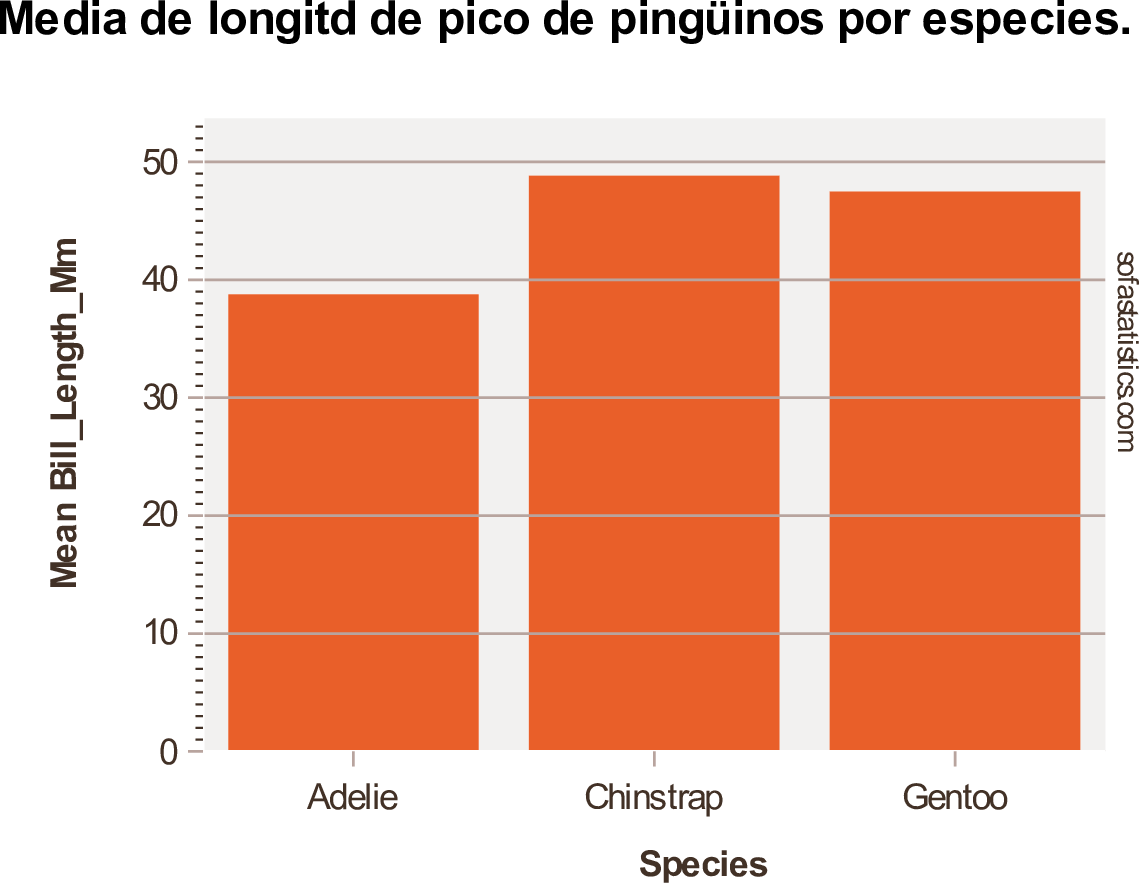
\includegraphics[width=0.7\textwidth]{1.png}
    \end{figure}

    \item \textbf{JASP:}
    \begin{figure}[H]
        \centering
        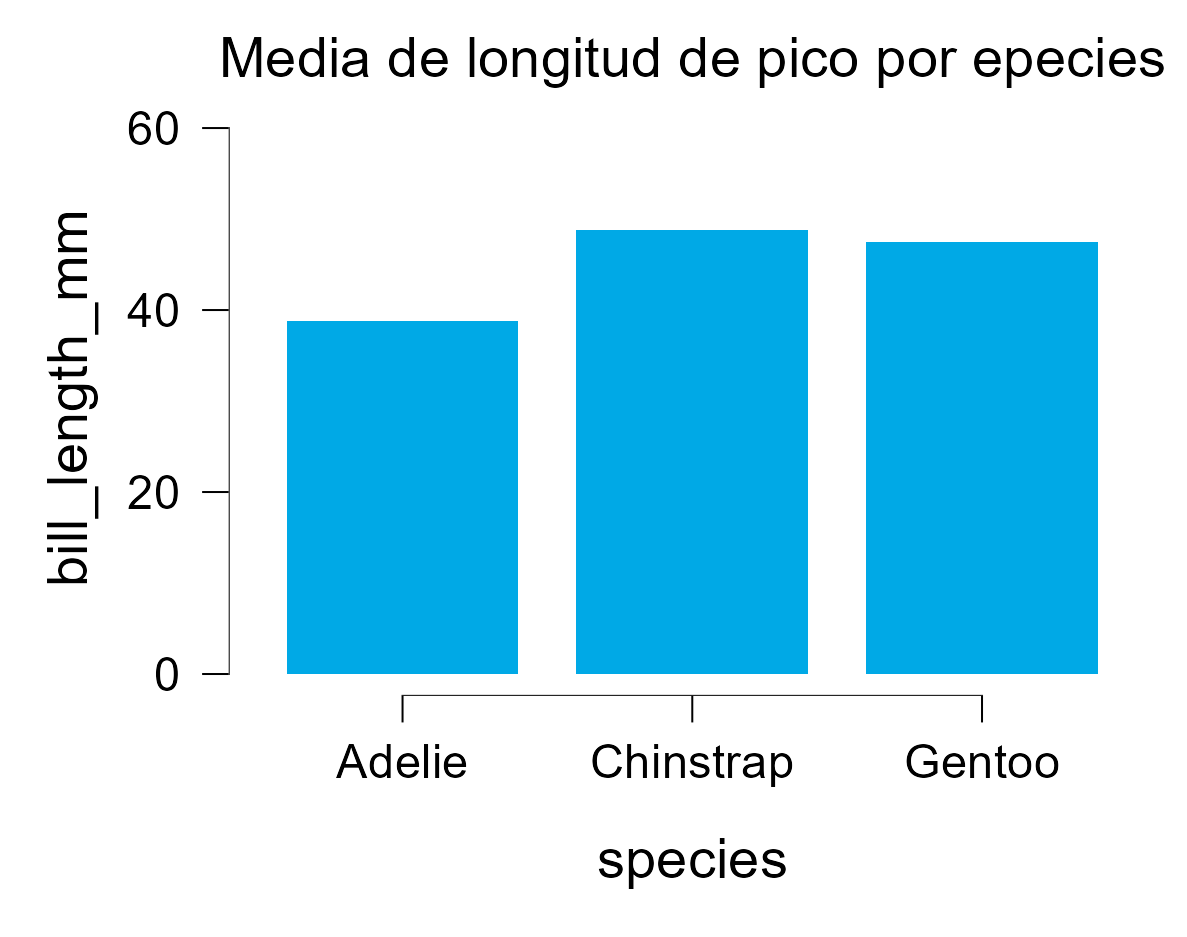
\includegraphics[width=0.7\textwidth]{2.png}
    \end{figure}
\end{itemize}

\subsection{Librerías de programación}
\begin{itemize}
    \item \textbf{Matplotlib (Python):}
    \begin{figure}[H]
        \centering
        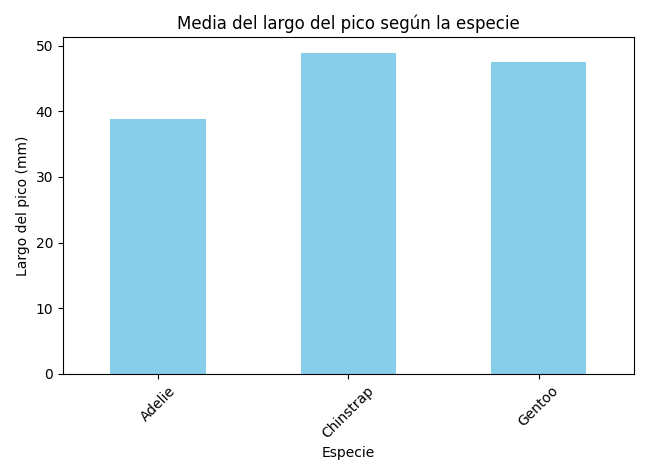
\includegraphics[width=0.7\textwidth]{3.png}
    \end{figure}

    \item \textbf{Plotly (Python):}
    \begin{figure}[H]
        \centering
        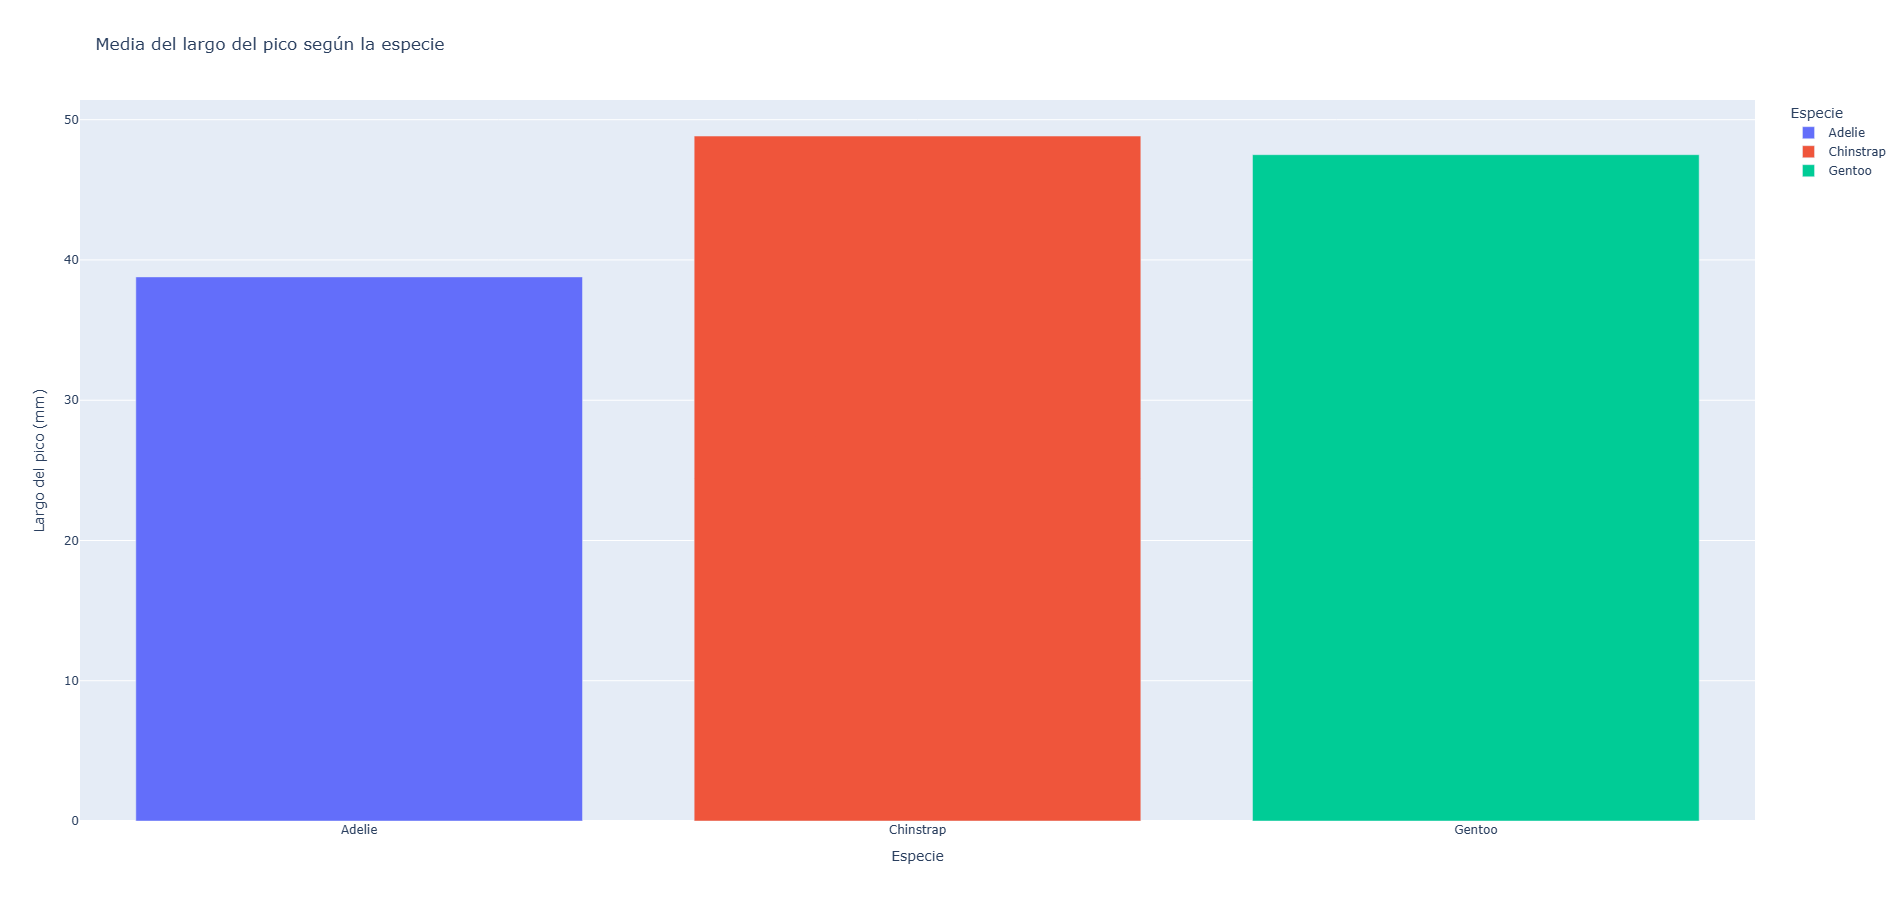
\includegraphics[width=0.7\textwidth]{4.png}
    \end{figure}
\end{itemize}

\newpage

\subsection{Herramientas online}
Hay que tener en cuenta que estas herramientas no suelen tener herramientas de calculo, por lo que se deben introducir los datos ya resumidos.
\begin{itemize}
    \item \textbf{Datawrapper:}
    \begin{figure}[H]
        \centering
        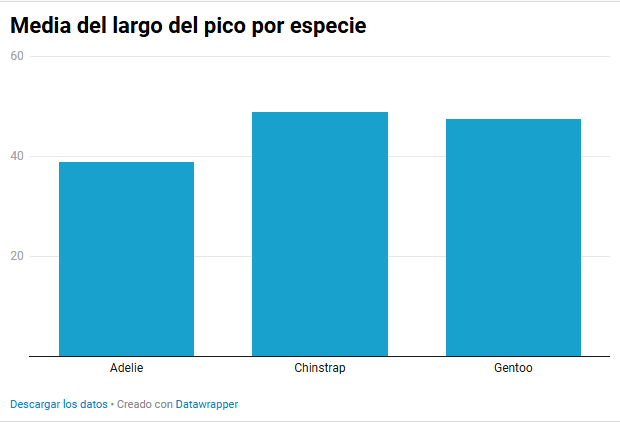
\includegraphics[width=0.7\textwidth]{5.png}
    \end{figure}

    \item \textbf{Canva:}
    \begin{figure}[H]
        \centering
        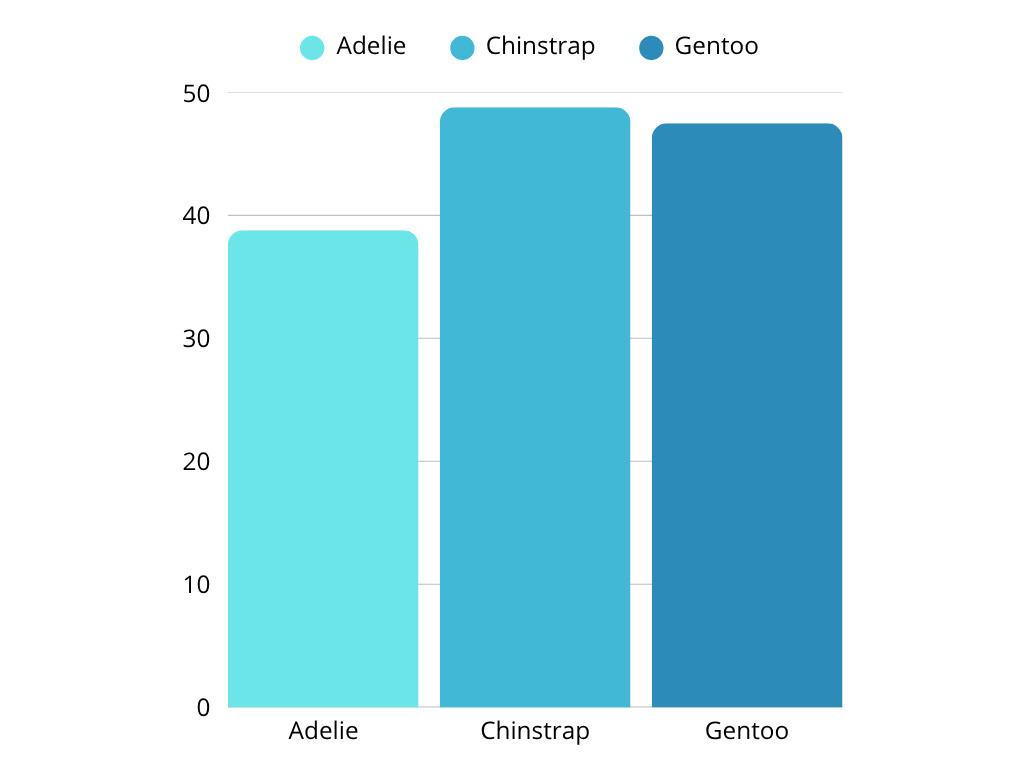
\includegraphics[width=0.7\textwidth]{6.png}
    \end{figure}
\end{itemize}

\newpage

\section{Reflexión final}

\begin{itemize}
    \item \textbf{Investigador en ciencias sociales:} Probablemente prefiera \textbf{JASP} o \textbf{SOFA Statistics}, por su facilidad de uso y enfoque estadístico.
    \item \textbf{Empresa que quiere difundir resultados en redes sociales:} Herramientas como \textbf{Canva} o \textbf{Datawrapper} destacan por su estética y facilidad para compartir visualizaciones online.
    \item \textbf{Analista de datos que trabaja en Python:} Librerías como \textbf{Matplotlib} o \textbf{Plotly} son ideales, ya que permiten gran personalización y análisis avanzado, además de integración con otros procesos de datos.
\end{itemize}

\section{Conclusión}
Cada tipo de herramienta tiene fortalezas específicas según el contexto: las estadísticas de código abierto son más adecuadas para análisis científico, las librerías de programación ofrecen control y personalización, y las herramientas online facilitan la difusión visual y atractiva de los datos.

\end{document}
